\documentclass{article}
\usepackage[minionint,mathlf,textlf]{MinionPro} % To gussy up a bit
\usepackage[margin=1in]{geometry}
\usepackage{graphicx} % For .eps inclusion
%\usepackage{indentfirst} % Controls indentation
\usepackage[compact]{titlesec} % For regulating spacing before section titles
\usepackage{adjustbox} % For vertically-aligned side-by-side minipages
\usepackage{array, mathrsfs, mathrsfs, mhchem, amsmath} % For centering of tabulars with text-wrapping columns
\usepackage{hyperref, chemfig}
\usepackage{subfigure}
\usepackage[autolinebreaks,framed,numbered]{mcode}
\newcommand{\Lapl}{\mathscr{L}}

\pagenumbering{gobble} 
\setlength\parindent{0 cm}
\begin{document}
\large

\section*{Recap of Turing patterns with note on stationary waves in two dimensions}

In the last question on this week's problem set, you'll be asked to determine which modes will be unstable for a given field size. (The goal of the problem is to show that more stripes will appear as an organism grows.) That question is framed so that it can be solved using the simplifying assumption that the relevant length scale $L$ is the distance from one corner of the field to the other. This works well for explaining the number of stripes in a long, thin domain, but does not explain the transition from a striped pattern to a spotted one as the organism grows fatter.\\

To explain the spots, we should consider perturbations of the form:
\[ \begin{pmatrix} \alpha\\ \beta \end{pmatrix} = \begin{pmatrix} \alpha_0\\ \beta_0 \end{pmatrix} e^{\lambda t} e^{iqx} e^{iry} \]

We will plug this solution into our reaction-diffusion equation on the plane:
\[ \frac{\partial}{\partial t} \begin{pmatrix} \alpha\\ \beta \end{pmatrix} = \mathbf{C} \begin{pmatrix} \alpha\\ \beta \end{pmatrix} + \mathbf{D} \nabla^2 \begin{pmatrix} \alpha\\ \beta \end{pmatrix} \]
$\nabla^2$ is the Laplace operator. In one dimension, it is simply the second spatial derivative. On the Cartestian plane, it is:
\[ \nabla^2 = \frac{\partial^2}{\partial x^2} + \frac{\partial^2}{\partial y^2} \]
Plugging in, calculating the derivatives, and combining terms, we have:
\begin{eqnarray}
\left[ \mathbf{C} - \left( q^2 + r^2 \right) \mathbf{D} - \lambda \mathbf{I} \right] \begin{pmatrix} \alpha_0\\ \beta_0 \end{pmatrix} = 0 \implies \left|\mathbf{C} - \left( q^2 + r^2 \right) \mathbf{D}  - \lambda \mathbf{I} \right| = 0 \label{eqn:twodeigenvalue}
\end{eqnarray}
Expanding out the determinant gives a quadratic expression for $\lambda$. We need at least one of the $\lambda_i$ to be positive for the system to be unstable, however, the $\lambda_i$ are centered around a negative number. Therefore we need a large discriminant term to push the large solution to a positive value. Specifically, we need\footnote{See Lecture 29 notes or the spatial modeling chapter by Iglesias for the full version of an analogous derivation.}:
\begin{eqnarray}
 \textrm{det} \left( \mathbf{C} \right) - \left(q^2 + r^2 \right) \left(c_{11}D_B + c_{22} D_A \right) + \left(q^2 + r^2 \right)^2 D_A D_B < 0 \label{eqn:twod}
 \end{eqnarray}
As in the one-dimensional case, the wavenumbers $q$ and $r$ cannot assume just any value. Consider a patterning field shaped like the round surface of a cylinder.

\begin{center}
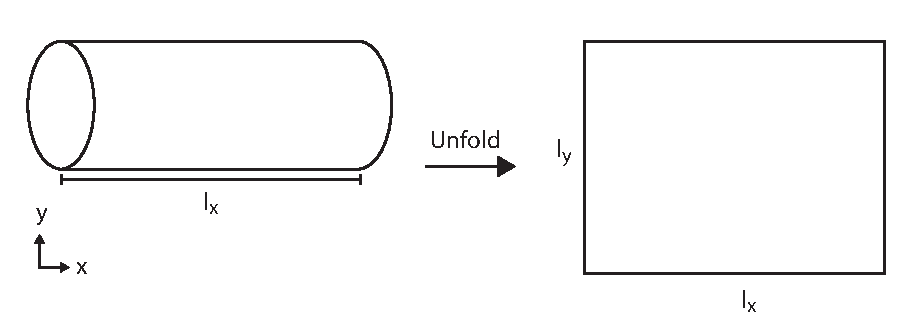
\includegraphics[width=0.5\textwidth]{geometry.pdf}
\end{center}

We could cut this surface and lay it flat: it would have a length $\ell_x$ equal to the length of the cylinder and a height $\ell_y$ equal to the circumference of the cylinder. The ``boundaries" at $x=0$ and $x=\ell_x$ are reflective: we therefore require that $\partial_{xx}$ be zero there. The allowable modes in this dimension therefore include half-waves. However, the ``boundaries" at $y=0$ and $y=\ell_y$ must have equal values, so only full waves are allowed in the $y$ direction. Thus:
\[ q_n = \frac{\pi \, n}{\ell_x} \hspace{1 cm} \textrm{and} \hspace{1 cm} r_m = \frac{2 \, \pi \, m}{\ell_y} , \hspace{1 cm} n, m \in \mathbb{N^0} \]

\begin{center}
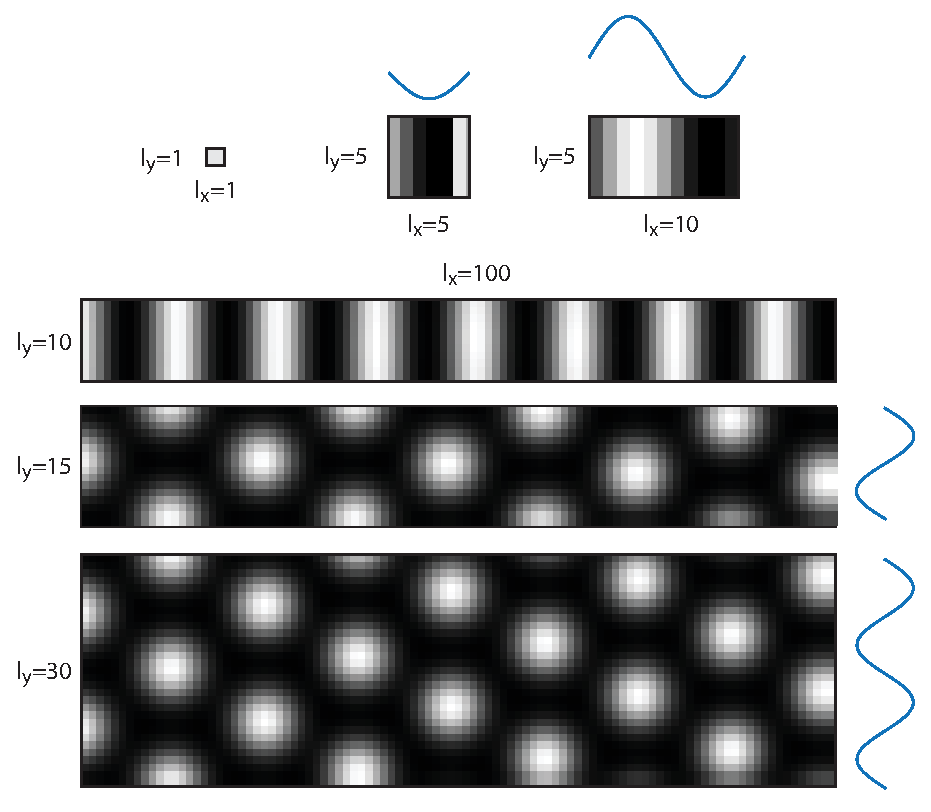
\includegraphics[width=0.5\textwidth]{first_modes_excited.pdf}
\end{center}

To find which modes can be excited for given $\ell_x$ and $\ell_y$, we can plug trial combinations of $q_n$ and $r_m$ into inequality \ref{eqn:twod} and check whether it is satisfied. Multiple combinations may satisfy the expression: in this case, the one which will ``win" at long times is the one with the largest eigenvalue, which we could determine using equation \ref{eqn:twodeigenvalue}.

\subsection*{Aside: non-stationary spatial waves}

One of the two lectures cut from this year's course was on symmetry and symmetry breaking. We would have covered an example where spatial oscillations are used to identify the center of the \textit{E. coli} cell, where the septum will form. The basic principle is that oscillations in MinD from one pole to the opposite leave a region in the middle where the average concentration of MinD is relatively low: it is in this region that the contractile FtsZ ring will form at cell division.\\

The Min system is one of the rare few that can be reconstituted \textit{in vitro} (Loose et al., 2008 and Zieske and Schwille, 2014). Zieske and Schwille induce these oscillations in compartments of varying size, demonstrating that if the dimensions are changed the number of regions where average MinD concentration is low will change. This strikingly demonstrates the dependency of the system on the dimensions of the cell. [Videos from Zieske and Schwille, 2014.]

\section*{Introduction to modularity and evolvability}

Critical genes are not at liberty to explore sequence space freely: no mutation in them will persist if it impairs their function. This means that these genes can become trapped in ``local maxima" of performance or fail to gain new functions that interfere with their original one. This limitation can be bypassed, however, via random gene duplication.\\

After gene duplication, as long as one copy of the gene continues to perform its essential function, the other paralog is freed of selective pressure. A typical outcome is that the unnecessary paralog becomes a non-functional pseudogene and over time is lost entirely. However, with luck, this paralog might instead acquire a new and useful function through mutation. This strategy for acquiring new functionality through gene duplication and subsequent divergence was first proposed by Susumu Ohno (1970) and nowadays has strong support from sequence analysis.\\

The notion that strong selection to maintain a current function is likely to interfere with evolution of a new function is not simply a narrative: in several specific systems it has been demonstrated directly. Consider for example TEM-1 $\beta$-lactamase, the ampicillin resistance-conferring \textit{bla} gene found on virtually every bacterial plasmid map. Stiffler et al. (2015) recently explored all amino acid substitution in TEM-1 \textit{exhaustively} (19 alternatives at each of nearly 300 residues) and found that 106 of them allow TEM-1 to better neutralize cefotaxime, another antibiotic. Unfortunately, most of these mutations also interfere with the enzyme's ability to neutralize ampicillin as evidenced by a fitness defect when grown on ampicillin. The implication is that it would be relatively difficult for the gene to evolve cefotaxime neutralization while undergoing selection for ampicillin resistance. This is a case where gene duplication and subsequent relief of selection on one paralog would facilitate acquisition of a new function. 

\begin{center}
\includegraphics[width=0.5\textwidth]{stiffler_graphic.pdf}
\end{center}


\section*{Two-component systems}

One gene family where this mode of evolution is especially apparent are the two-component signaling systems. (The signaling lecture was unfortunately canceled this year due to weather, so we will instead discuss that system here.) Unlike the MAP kinase systems which have appeared often in the course, two-component systems consist of only a receptor (called a histidine kinase) and the response regulator, a signaling effector. The receptor gets this name because it controls the phosphorylation state of its response regulator by transferring a phosphate from a histidine residue to the RR in a signaling-dependent manner. When no signaling is occurring, it may also act as a phosphatase.

\begin{center}
\includegraphics[width=0.5\textwidth]{two_component_diagram.pdf}
\end{center}

Whereas the serine/threonine and tyrosine receptor families have expanded substantially in eukaryotes, histidine kinases are the major expanded family in bacteria: some species have as many as 200 two-component pathways, though most have only around 30. In many cases both a histidine kinase and its corresponding response regulator are found in a single operon, facilitating duplication of the pair. Despite their common origins, these two-component pathways are very effective at avoiding crosstalk.  To show this, Skerker et al. (2005) added $^{32}$P-labeled ATP to purified histidine kinases, which transferred the labeled phosphate to their histidines. They then added the same response regulator to each reaction and checked for transfer from the HK to the response regulator after 10 seconds or one hour. Only the correct pair showed transfer on the fast timescale. (Slower reactions were apparent for a pair isolated in vitro, but would likely not be relevant physiologically due to competition between response regulators within the cell.)

\begin{center}
\includegraphics[width=0.8\textwidth]{skerker2005.pdf}
\end{center}

Attaining specificity of interactions following duplication and divergence is a major concern for the neofunctionalization by duplication and divergence. Even before the first HK-RR crystal structure was solved, the Laub lab was searching for the interactions between histidine kinases and their response regulators that conferred specificity. These proteins had accumulated many sequence differences over a very long period of divergence, so that the relevant changes could not be identified simply by alignment and inspection. Skerker et al. (2008) approached this problem computationally, taking advantage of the fact that mutations at the interaction interface on one partner might be compensated by mutations on the other. Thirteen hundred HK-RR sequence pairs were known to science at that time: within this dataset, perhaps the same compensating mutations would have arisen independently multiple times.\\

The authors used a metric called mutual information to search for cases where knowing the amino acid at one residue on one partner gave a better-than-chance prediction of the amino acid at a residue on the other partner. If $p_i$ is the probability of finding amino acid $i$ at residue $x$ on the HK, and $p_j$ is the proboably of finding amino acid $j$ at residue $y$ on the RR, and $p_{ij}$ is the probability of both occurring, then
\[ \textrm{MI } = \sum_{i=1}^{20} \sum_{j=1}^{20} p_{ij} \ln \left( \frac{p_{ij}}{p_i p_j} \right) \]
If the two events are independent, then $p_{ij} \approx p_i p_j$ and the ratio within the logarithm is 1, so the mutual information is zero. Additional co-occurrence would elevate the score.

\begin{center}
\includegraphics[width=0.6\textwidth]{mi.pdf}
\end{center}

This purely mathematical approach identified several pairs of sites that spanned these two proteins which appeared to be ``evolving together," so that certain sequence combinations were much more common than others. Mapping these residues to the closest cognate structure available at that time, the authors found that they seemed to fall at the interface between the two partners just as one would predict.

\begin{center}
\includegraphics[width=0.4\textwidth]{spo0f.pdf}
\end{center}

Following duplication, specificity of the new pair for the other could evolve in one of two broad ways. One protein could acquire a mutation by which it loses the ability to interact with its partner (creating a non-functional interaction), and then the partner could happen to evolve a compensatory mutation before either becomes a pseudogene. Alternatively, it might be possible for the specificity residues to mutate in some order by which the two partners never lose the ability to interact with one another. Determining which of these is more likely requires understanding the range of sequence combinations that confer specificity.\\

A related question is how well two-component systems have sampled the space of sequences conferring specificity. Do specificity sequences become trapped in local minima, or are extant two-component systems representative of the full range of possible sequence combinations conferring specificity?\\

In a recent attempt to address these question, Pedgornaia and Laub (2015) generate variants of the histidine kinase PhoQ that differ from the wildtype sequence at four residues in the interaction interface. They estimate that all 160,000 possible amino acid sequence variants are covered by their random library. To assess whether these variants are functional, they select cells which express a fluorescent reporter activated by PhoQ's response regulator, PhoP. (Under these conditions, if the PhoQ is not specific, it may transfer its phosphate to other response regulators in the cell which will decrease reporter expression.) The authors find a vast network of sequences which differ from each other by only one amino acid. However, all known PhoQ sequences fall within one region of this network. This may reflect constraints in the ability to mutate from some amino acids to others (some changes require only one base pair mutation; others, more).

\begin{center}
\includegraphics[width=0.8\textwidth]{podgornaia.pdf}
\end{center}

\end{document}